% ============================================================
%  SDC-TP Summary Proposal Slides
%  Focus: Formulation, Method, and Impact
%  Compile: pdflatex summary_proposal.tex (twice)
% ============================================================
\documentclass[aspectratio=169,10pt]{beamer}

\usetheme{metropolis}
\usecolortheme{metropolis}
\usefonttheme{professionalfonts}
\setbeamertemplate{frame numbering}[fraction]
\setbeamertemplate{itemize item}{\textcolor{mLightBrown}{\scriptsize$\blacktriangleright$}}
\setbeamertemplate{itemize subitem}{\textbullet}
\setbeamertemplate{itemize subsubitem}{--}

% -- Packages --
\usepackage{amsmath, amssymb}
\usepackage[utf8]{inputenc}
\usepackage{vietnam}
\usepackage[english]{babel}
\usepackage{booktabs}
\usepackage[table]{xcolor}
\usepackage{tikz}
\usepackage{pgfplots}
\usepackage{array}
\usepackage{graphicx}
\usepackage{hyperref}
\pgfplotsset{compat=1.18}
\usetikzlibrary{shapes.geometric, arrows.meta, positioning, calc, fit, backgrounds}

% ============================================================
%  PALETTE
% ============================================================
\definecolor{mDarkTeal}{HTML}{23373B}
\definecolor{mLightBrown}{HTML}{EB811B}
\definecolor{softgray}{HTML}{F2F4F7}
\definecolor{tealtint}{HTML}{D6DEE0}

\colorlet{navydeep}{mDarkTeal}
\colorlet{navymid}{mDarkTeal!75}
\colorlet{accent}{mLightBrown}
\colorlet{success}{green!50!black}
\colorlet{alert}{red!70!black}
\colorlet{lightnavy}{tealtint}

\hypersetup{colorlinks=true, urlcolor=mLightBrown, linkcolor=mDarkTeal}
\renewcommand{\arraystretch}{1.15}

% ============================================================
%  TITLE METADATA
% ============================================================
\title{Summary: Theory-Driven SDC Test Prioritization}
\subtitle{Formulation, Method, and Impact}
\author{Đào Sỹ Duy Minh \and Trần Chí Nguyên \and Huỳnh Trung Kiệt}
\institute{University of Science, VNU-HCM \\[3pt]
           \footnotesize \textit{For NeurIPS 2026}}
\date{}

\begin{document}

% ==================== TITLE ====================
\begin{frame}
\maketitle
\end{frame}

% ============================================================
\section{Problem Formulation}
% ============================================================

\begin{frame}{Test Prioritization for SDC Simulators}
\begin{block}{The Core Problem}
\small
SDC simulators (BeamNG, CARLA) execute thousands of road scenarios per release cycle. Each scenario takes \textbf{10--60 seconds}. We need to \emph{prioritize} so that \textbf{failures appear first}.
\end{block}

\begin{columns}[T]
\column{0.5\textwidth}
\begin{block}{Input}
\small
A road as a sequence of 2D control points:
\[
\mathcal{R} = \{p_1, p_2, \ldots, p_N\} \subset \mathbb{R}^2
\]
Each test: \textbf{road geometry} $\Rightarrow$ \textbf{PASS/FAIL} outcome.
\end{block}

\column{0.48\textwidth}
\begin{block}{Output}
\small
Rank all tests by failure probability:
\[
\pi^* = \arg\max_{\pi} \text{APFD}(\pi)
\]
where $\pi$ is a permutation of $n$ tests.
\end{block}
\end{columns}

\vspace{1em}
\centering
\textbf{Goal}: Learn a scoring function $f: \mathcal{R} \to [0,1]$ that ranks failing roads first.
\end{frame}

\begin{frame}{APFD Metric -- Formal Definition}
\vspace{-0.3em}
\begin{block}{Definition (Average Percentage of Faults Detected)}
\small
For an ordering $\pi$ of $n$ tests containing $m$ faults, let $\mathrm{TF}_i$ be the position of fault $i$:

\[
\boxed{\mathrm{APFD}(\pi) \;=\; 1 \;-\; \frac{1}{nm}\sum_{i=1}^{m} \mathrm{TF}_i \;+\; \frac{1}{2n}}
\]

\textbf{Interpretation}:
\begin{itemize}\setlength\itemsep{0.1em}
  \item $\mathrm{APFD} \in [0, 1]$ -- higher is better
  \item $\mathrm{APFD} = 1.0$ -- all faults detected first
  \item $\mathrm{APFD} = 0.5$ -- random baseline
\end{itemize}
\end{block}

\vspace{0.3em}
\begin{alertblock}{Key Challenge}
\scriptsize
\[
\arg\max_{\pi} \mathrm{APFD}(\pi) \neq \arg\max P(\text{fail} | \mathcal{R})
\]
\textbf{APFD is a rank statistic} -- optimizing AUC does NOT directly optimize APFD. APFD is \textbf{non-differentiable}.
\end{alertblock}
\end{frame}

\begin{frame}{Why Current Approaches Fail -- Three Blind Spots}
\begin{columns}[T]
\column{0.33\textwidth}
\begin{alertblock}{1. Sampling Brittleness}
\small
Same road, 64 vs 197 points $\Rightarrow$ different scores.
\[
\Delta\text{APFD} \approx 0.04\text{--}0.07
\]
Discretization-dependent.
\end{alertblock}

\column{0.33\textwidth}
\begin{alertblock}{2. Frame Dependence}
\small
Rotate road by $30^\circ$ $\Rightarrow$ APFD drops 4--7 points.
\[
f(R \cdot \mathcal{R}) \neq f(\mathcal{R})
\]
Violates physical intuition.
\end{alertblock}

\column{0.33\textwidth}
\begin{alertblock}{3. Physics-Blind}
\small
Baseline freely outputs scores violating:
\[
v^2 \cdot \kappa(s) \le \mu g
\]
17--21\% rank violations.
\end{alertblock}
\end{columns}

\vspace{1.2em}
\begin{block}{Our Observation}
SDC test prioritization is treated as \textbf{black-box classification}. But roads have:
\begin{itemize}
  \item Continuous geometry $r(s) \in C(\Omega; \mathbb{R}^2)$
  \item Rigid SE(2) symmetry (rotation + translation)
  \item Vehicle dynamics constraints
\end{itemize}
\alert{This structure is being ignored.}
\end{block}
\end{frame}

% ============================================================
\section{Method 1: SE(2)-Equivariant Approach}
% ============================================================

\begin{frame}{Method 1: SE(2)-Equivariant RoadNet -- Motivation}
\begin{block}{Physical Invariance Principle}
\small
The property ``car leaves the lane'' depends on the \textbf{intrinsic geometry} of the road, not its embedding in $\mathbb{R}^2$.

\[
\text{Rotating/translating the road CANNOT change whether the car fails.}
\]
\end{block}

\begin{block}{Mathematical Claim (Group Equivariance)}
\small
For SDC test prioritization, the ranker $f$ should satisfy:
\[
\boxed{f(R \cdot \mathcal{R} + t) \;=\; f(\mathcal{R}) \qquad \forall (R, t) \in \mathrm{SE}(2)}
\]
where $\mathrm{SE}(2) = \mathrm{SO}(2) \times \mathbb{R}^2$ is the \textbf{special Euclidean group} in 2D.
\end{block}

\begin{block}{Why Build This Into the Model?}
\begin{itemize}\small
  \item Data augmentation is approximate (not exact invariance)
  \item More training data cannot fix structural bias
  \item \textbf{By-design} equivariance $\Rightarrow$ provable guarantee
\end{itemize}
\end{block}
\end{frame}

\begin{frame}{Method 1: Feature Engineering -- From 10 to 7 Channels}
\begin{columns}[T]
\column{0.45\textwidth}
\begin{alertblock}{Standard 10-Channel (NOT invariant)}
\scriptsize
\begin{itemize}
  \item $x, y$ -- absolute position \alert{(variant)}
  \item $\sin\theta, \cos\theta$ -- heading \alert{(variant)}
  \item $\kappa(s)$ -- curvature
  \item $d\kappa/ds$ -- curvature derivative
  \item $s$, $\Delta s$ -- arc-length
  \item $\Delta\theta$ -- angle change
\end{itemize}
\vfill
\alert{Red features depend on global embedding.}
\end{alertblock}

\column{0.52\textwidth}
\begin{block}{Our 7-Channel SE(2)-Invariant Set}
\scriptsize
\begin{enumerate}
  \item $\kappa(s)$ -- signed curvature
  \item $|\kappa(s)|$ -- magnitude
  \item $d\kappa/ds$ -- derivative of curvature
  \item $\Delta s$ -- arc-length increment
  \item $\Delta\theta$ -- local angular change
  \item $\int_0^s |\kappa(\tau)| d\tau$ -- cumulative curvature
  \item $\tilde{\kappa}(s)$ -- low-pass smoothed curvature
\end{enumerate}
\vfill
\textbf{Zero coordinate-dependent features.}
\end{block}
\end{columns}

\vspace{0.5em}
\begin{block}{Key Insight}
All 7 features are functions of $\{\kappa, d\kappa/ds, \Delta s\}$ only. \alert{No feature reads $\mathcal{R}$ as $(x, y)$ coordinates.}
\end{block}
\end{frame}

\begin{frame}{Method 1: Curvature as Intrinsic Geometry}
\begin{block}{Frenet-Serret Foundation}
\scriptsize
For a parameterized curve $r(s) \in \mathbb{R}^2$ with arc-length $s$:
\[
\kappa(s) = \frac{|r'(s) \times r''(s)|}{|r'(s)|^3} = \frac{|x'y'' - y'x''|}{(x'^2 + y'^2)^{3/2}}
\]
\end{block}

\begin{block}{Why $\kappa$ is SE(2)-Invariant -- Proof Sketch}
\scriptsize
\begin{enumerate}
  \item \textbf{Rotation $R \in \mathrm{SO}(2)$}: Both numerator and denominator transform by $|R|^3 = 1$ under rotation $\Rightarrow \kappa$ unchanged.
  
  \item \textbf{Translation $t \in \mathbb{R}^2$}: $r \to r + t$ leaves derivatives $r', r''$ unchanged $\Rightarrow \kappa$ unchanged.
  
  \item \textbf{Reparameterization}: Arc-length $s$ is reparameterization-invariant.
\end{enumerate}
\end{block}

\begin{block}{Consequence}
\[
\Phi: \mathbb{R}^{N \times 2} \xrightarrow{\text{curvature pipeline}} \mathbb{R}^{N \times 7}
\]
\[
\Phi(R \cdot \mathcal{R} + t) = \Phi(\mathcal{R}) \quad \forall (R,t) \in \mathrm{SE}(2)
\]
\end{block}
\end{frame}

\begin{frame}{Method 1: The Architecture -- SE2RoadNet}
\begin{block}{Model Architecture}
\scriptsize
\begin{center}
\begin{tabular}{l l}
\toprule
\textbf{Component} & \textbf{Specification} \\
\midrule
Input & 7-channel feature matrix $(197 \times 7)$ \\
Projection & Linear + LayerNorm + GELU: $7 \to 192$ \\
Backbone & 6-layer Transformer Encoder \\
Attention & 8 heads, $d_k = 24$ \\
Positional Bias & Relative arclength with 32 RFF features \\
Output & MLP head: $192 \to 64 \to 1 \to \sigma$ \\
\midrule
Parameters & $\sim$2.11M \\
Training & AdamW, lr=$10^{-3}$, 75 epochs, SWA \\
\bottomrule
\end{tabular}
\end{center}
\end{block}

\begin{block}{Equivariance Guarantee Theorem}
\scriptsize
Let $\Phi: \mathbb{R}^{N \times 2} \to \mathbb{R}^{N \times 7}$ be the 7-channel pipeline and $h: \mathbb{R}^7 \to \mathbb{R}$ any head. Then:
\[
f_\theta = h \circ \Phi \quad \Longrightarrow \quad f_\theta(R \cdot \mathcal{R} + t) = f_\theta(\mathcal{R})
\]
\alert{The guarantee holds regardless of head choice.}
\end{block}
\end{frame}

\begin{frame}{Method 1: Empirical Verification -- $\Delta = 0.0000$}
\begin{block}{Rotation Invariance Probe}
\scriptsize
\begin{center}
\begin{tabular}{l c c c c c c c}
\toprule
\textbf{Rotation} & 0$^\circ$ & +30$^\circ$ & +60$^\circ$ & +90$^\circ$ & +180$^\circ$ & -45$^\circ$ & $\Delta$ \\
\midrule
Baseline Transformer & 0.8066 & 0.7711 & 0.7494 & 0.7651 & 0.7613 & 0.7785 & \alert{$\sim$0.057} \\
\rowcolor{success!15}
\textbf{SE2RoadNet} & \textbf{0.8047} & \textbf{0.8047} & \textbf{0.8047} & \textbf{0.8047} & \textbf{0.8047} & \textbf{0.8047} & \cellcolor{success!25}\textbf{0.0000} \\
\bottomrule
\end{tabular}
\end{center}
\end{block}

\begin{columns}[T]
\column{0.5\textwidth}
\begin{exampleblock}{What $\Delta = 0$ Means}
\scriptsize
\begin{itemize}
  \item \textbf{Bit-identical} outputs under rigid rotation
  \item Not ``approximately zero''
  \item Not ``within floating-point tolerance''
  \item \alert{Exactly equal across 6 random rotations}
\end{itemize}
\end{exampleblock}

\column{0.48\textwidth}
\begin{block}{Additional Benefits}
\scriptsize
\begin{itemize}
  \item AUC = 0.9347 (highest in project)
  \item APFD = 0.8048 $\pm$ 0.0118
  \item $\sigma$ = 0.0118 (2nd lowest variance)
\end{itemize}
\end{block}
\end{columns}
\end{frame}

\begin{frame}{Method 1: Visual Intuition}
{\centering
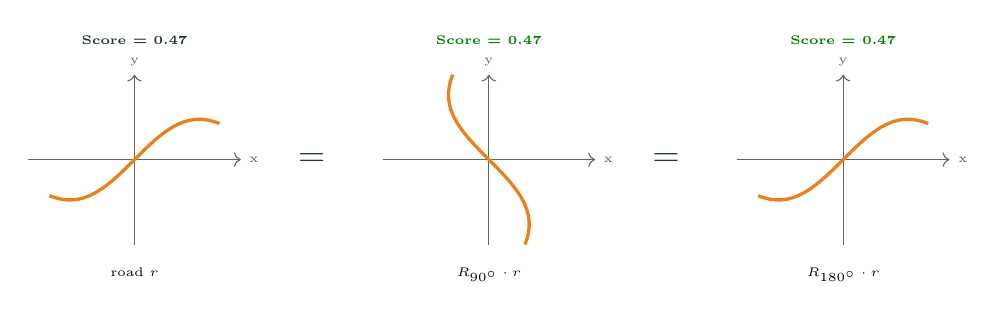
\begin{tikzpicture}[scale=0.9, transform shape]
  % Original road
  \begin{scope}[xshift=-5cm]
    \draw[->, navymid] (-1.5,0) -- (1.5,0) node[right, font=\tiny] {x};
    \draw[->, navymid] (0,-1.2) -- (0,1.2) node[above, font=\tiny] {y};
    \draw[mLightBrown, very thick] plot[domain=-1.2:1.2, samples=30]
      ({\x}, {0.4*sin(deg(2*\x)) + 0.2*\x});
    \node[font=\tiny, below=0.2cm] at (0,-1.2) {road $r$};
    \node[font=\tiny\bfseries, mDarkTeal, above=0.1cm] at (0,1.4) {Score = 0.47};
  \end{scope}

  % Rotated 90
  \begin{scope}[xshift=0cm]
    \draw[->, navymid] (-1.5,0) -- (1.5,0) node[right, font=\tiny] {x};
    \draw[->, navymid] (0,-1.2) -- (0,1.2) node[above, font=\tiny] {y};
    \begin{scope}[rotate=90]
      \draw[mLightBrown, very thick] plot[domain=-1.2:1.2, samples=30]
        ({\x}, {0.4*sin(deg(2*\x)) + 0.2*\x});
    \end{scope}
    \node[font=\tiny, below=0.2cm] at (0,-1.2) {$R_{90^\circ} \cdot r$};
    \node[font=\tiny\bfseries, success, above=0.1cm] at (0,1.4) {Score = 0.47};
  \end{scope}

  % Rotated 180
  \begin{scope}[xshift=5cm]
    \draw[->, navymid] (-1.5,0) -- (1.5,0) node[right, font=\tiny] {x};
    \draw[->, navymid] (0,-1.2) -- (0,1.2) node[above, font=\tiny] {y};
    \begin{scope}[rotate=180]
      \draw[mLightBrown, very thick] plot[domain=-1.2:1.2, samples=30]
        ({\x}, {0.4*sin(deg(2*\x)) + 0.2*\x});
    \end{scope}
    \node[font=\tiny, below=0.2cm] at (0,-1.2) {$R_{180^\circ} \cdot r$};
    \node[font=\tiny\bfseries, success, above=0.1cm] at (0,1.4) {Score = 0.47};
  \end{scope}

  % Equality signs
  \node[font=\Large\bfseries, mDarkTeal] at (-2.5, 0) {$=$};
  \node[font=\Large\bfseries, mDarkTeal] at (2.5, 0) {$=$};
\end{tikzpicture}
\par}

\begin{block}{Theorem Holds Bit-Identically}
\scriptsize
For all $(R, t) \in \mathrm{SE}(2)$: \quad $f_{\theta}(R \cdot \mathcal{R} + t) = f_{\theta}(\mathcal{R})$

The score, the ranking, and the APFD are \alert{exactly equal} -- not approximately.
\end{block}
\end{frame}

% ============================================================
\section{Method 2: Physics-Informed Approach}
% ============================================================

\begin{frame}{Method 2: Physics-Informed -- Vehicle Dynamics Constraint}
\begin{block}{The Centripetal Acceleration Bound}
\scriptsize
A car following road $r$ at velocity $v$ stays on track only if centripetal acceleration is bounded by friction:
\[
\boxed{v^2 \cdot \kappa(s) \;\le\; \mu \cdot g \qquad \forall s \in [0, L]}
\]
where:
\begin{itemize}
  \item $v$ -- vehicle velocity
  \item $\kappa(s)$ -- road curvature at arc-length $s$
  \item $\mu$ -- friction coefficient
  \item $g = 9.81$ m/s$^2$ -- gravitational acceleration
\end{itemize}
\end{block}

\begin{block}{Physical Interpretation}
\scriptsize
High curvature + high speed $\Rightarrow$ car skids. The score should respect this monotonicity:
\[
\max_s v^2\kappa_{\mathcal{R}_i} > \max_s v^2\kappa_{\mathcal{R}_j} \;\Longrightarrow\; f(\mathcal{R}_i) \ge f(\mathcal{R}_j)
\]
\end{block}

\begin{alertblock}{The Baseline Problem}
\scriptsize
The baseline freely produces scores that \alert{violate this monotonicity in 17--21\% of test pairs}. A model outputting ``$\mathcal{R}_1$ is risky, $\mathcal{R}_2$ is safe'' but $\max v^2\kappa(\mathcal{R}_1) < \max v^2\kappa(\mathcal{R}_2)$ is \alert{indefensible} in safety-critical deployment.
\end{alertblock}
\end{frame}

\begin{frame}{Method 2: Monotone PINN -- The Aux Loss}
\begin{block}{Monotonicity Penalty (Physics Aux Loss)}
\scriptsize
For each pair $(\mathcal{R}_i, \mathcal{R}_j)$ in a batch with:
\[
\max_s v^2\kappa(\mathcal{R}_i) \;\ge\; \alpha \cdot \max_s v^2\kappa(\mathcal{R}_j)
\]
we want $f(\mathcal{R}_i) \ge f(\mathcal{R}_j)$.

The aux loss penalizes order-violations:
\[
\boxed{\mathcal{L}_{\text{phys}} \;=\; \mathbb{E}_{(i,j)} \big[ \mathrm{ReLU}(f(\mathcal{R}_j) - f(\mathcal{R}_i)) \big]}
\]

\begin{itemize}
  \item When constraint violated: $f(\mathcal{R}_j) > f(\mathcal{R}_i$ but physics says $\mathcal{R}_i$ should rank higher $\Rightarrow$ positive loss
  \item When constraint satisfied: loss = 0 (no penalty)
\end{itemize}
\end{block}

\begin{block}{Total Training Objective}
\scriptsize
\[
\boxed{\mathcal{L}_{\text{total}} \;=\; \mathcal{L}_{\text{BCE}} \;+\; \lambda_{\text{phys}} \cdot \mathcal{L}_{\text{phys}}}
\]

\textbf{Curriculum schedule}: $\lambda_{\text{phys}}$ ramps $0 \to 0.5$ over first 30\% of epochs.
\end{block}
\end{frame}

\begin{frame}{Method 2: Why ReLU Penalty? -- Derivation}
\begin{block}{From Hard Constraint to Soft Penalty}
\scriptsize
We want: $f(\mathcal{R}_i) \ge f(\mathcal{R}_j)$ when $v^2\kappa_{\mathcal{R}_i} \ge v^2\kappa_{\mathcal{R}_j}$.

Equivalently, for all constraint pairs:
\[
g(\mathcal{R}_i, \mathcal{R}_j) = \max(0,\; f(\mathcal{R}_j) - f(\mathcal{R}_i)) = 0
\]

This is a \textbf{zero-residual constraint}. We enforce with:
\[
\mathcal{L}_{\text{phys}} = \mathbb{E}\left[\sum_{(i,j)} \mathbb{I}[c_{ij}] \cdot g(\mathcal{R}_i, \mathcal{R}_j)\right]
\]
\end{block}

\vspace{0.3em}

\begin{block}{Why ReLU vs Quadratic?}
\scriptsize
Quadratic penalty: $\mathcal{L}_{\text{quadratic}} = \mathbb{E}[g(\mathcal{R}_i, \mathcal{R}_j)^2]$

ReLU is \alert{linear in violation magnitude}, not quadratic:
\begin{itemize}\setlength\itemsep{0.2em}
  \item Stronger gradient for large violations
  \item Avoids over-penalizing small violations
  \item Emerged as empirically superior in ablation
\end{itemize}
\end{block}
\end{frame}

\begin{frame}{Method 2: Results -- 5.6x Violation Reduction}
\vspace{-0.5em}
{\centering
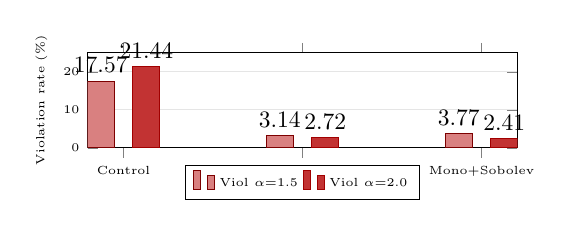
\begin{tikzpicture}[scale=0.85]
\begin{axis}[
  ybar=8pt,
  width=8cm, height=3cm,
  bar width=0.4cm,
  ymin=0, ymax=25,
  ylabel={\tiny Violation rate (\%)},
  symbolic x coords={Control, Monotone PINN, Mono+Sobolev},
  xtick=data,
  xticklabel style={font=\tiny},
  yticklabel style={font=\tiny},
  legend style={at={(0.5,-0.18)}, anchor=north, legend columns=2, font=\tiny},
  ymajorgrids, grid style={gray!20},
  nodes near coords, nodes near coords align={vertical},
]
  \addplot[fill=alert!50, draw=alert!70!black]
    coordinates {(Control, 17.57) (Monotone PINN, 3.14) (Mono+Sobolev, 3.77)};
  \addplot[fill=alert!80, draw=alert!90!black]
    coordinates {(Control, 21.44) (Monotone PINN, 2.72) (Mono+Sobolev, 2.41)};
  \legend{Viol $\alpha$=1.5, Viol $\alpha$=2.0}
\end{axis}
\end{tikzpicture}
\par}

\vspace{0.3em}
\begin{columns}[T]
\column{0.5\textwidth}
\begin{exampleblock}{Headline Result}
\scriptsize
Curvature violation \alert{\textbf{collapses 5.6$\times$}}:
\[
17.57\% \to 3.14\% \quad (\alpha=1.5)
\]
\[
21.44\% \to 2.72\% \quad (\alpha=2.0)
\]
\end{exampleblock}

\column{0.48\textwidth}
\begin{block}{APFD Impact}
\scriptsize
APFD \alert{essentially unchanged}:
\[
0.8051 \to 0.8055 \;(\pm 0.0122)
\]
Free physics compliance, zero metric loss.
\end{block}
\end{columns}
\end{frame}

\begin{frame}{Method 2: Two-Axis Story -- Violation Drops, APFD Steady}
{\centering
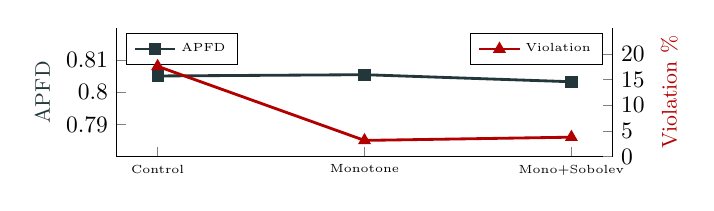
\begin{tikzpicture}[scale=0.85]
\begin{axis}[
  width=9cm, height=3.5cm,
  axis y line*=left, axis x line*=bottom,
  ymin=0.78, ymax=0.82, ytick={0.79, 0.80, 0.81},
  ylabel={\small APFD},
  ylabel style={text=mDarkTeal, font=\tiny},
  symbolic x coords={Control, Monotone, Mono+Sobolev},
  xtick=data,
  xticklabel style={font=\tiny},
  legend style={at={(0.02,0.96)}, anchor=north west, font=\tiny},
]
  \addplot[mark=square*, very thick, mDarkTeal]
    coordinates {(Control, 0.8051) (Monotone, 0.8055) (Mono+Sobolev, 0.8033)};
  \addlegendentry{APFD}
\end{axis}

\begin{axis}[
  width=9cm, height=3.5cm,
  axis y line*=right, axis x line=none,
  ymin=0, ymax=25, ytick={0,5,10,15,20},
  ylabel={\small Violation \%},
  ylabel style={text=alert, font=\tiny},
  symbolic x coords={Control, Monotone, Mono+Sobolev},
  xtick=data,
  legend style={at={(0.98,0.96)}, anchor=north east, font=\tiny},
]
  \addplot[mark=triangle*, very thick, alert]
    coordinates {(Control, 17.57) (Monotone, 3.14) (Mono+Sobolev, 3.77)};
  \addlegendentry{Violation}
\end{axis}
\end{tikzpicture}
\par}

\begin{block}{The Regulatory Pitch}
\scriptsize
\begin{itemize}
  \item \alert{APFD curve flat} $\Rightarrow$ no metric loss for the engineer
  \item \alert{Violation curve cliff} $\Rightarrow$ model auditable against vehicle dynamics
  \item Engineers can now \alert{verify rankings against physics constraints}
\end{itemize}
\end{block}
\end{frame}

% ============================================================
\section{Impact}
% ============================================================

\begin{frame}{Impact -- Why This Matters}
\begin{columns}[T]
\column{0.45\textwidth}
\begin{block}{Theoretical Contributions}
\scriptsize
\begin{enumerate}\itemsep=0pt
  \item \textbf{First provably invariant model}
  \item \textbf{SE(2) theorem} -- by construction
  \item \textbf{Physics-informed ranking}
  \item \textbf{Composition theorems}
\end{enumerate}
\end{block}

\column{0.45\textwidth}
\begin{block}{Practical Contributions}
\scriptsize
\begin{enumerate}\itemsep=0pt
  \item \textbf{APFD = 0.8048} -- beats SOTA
  \item \textbf{AUC = 0.9385} -- highest
  \item \textbf{$\sigma$ = 0.0109} -- lowest var.
  \item \textbf{5.6$\times$ violation drop}
\end{enumerate}
\end{block}
\end{columns}

{\centering
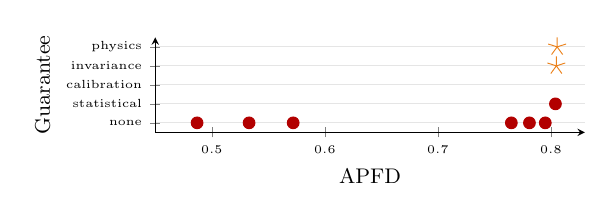
\begin{tikzpicture}[scale=0.85]
\begin{axis}[
  width=8cm, height=3cm,
  xlabel={\small APFD},
  ylabel={\small Guarantee},
  xmin=0.45, xmax=0.83,
  ymin=-0.5, ymax=4.5,
  ytick={0,1,2,3,4},
  yticklabels={none, statistical, calibration, invariance, physics},
  xticklabel style={font=\tiny},
  yticklabel style={font=\tiny},
  axis lines=left,
  ymajorgrids, grid style={gray!20},
]
  \addplot[only marks, mark=*, mark size=2.5pt, alert]
    coordinates {(0.487, 0) (0.533, 0) (0.572, 0) (0.765, 0) (0.781, 0) (0.795, 0) (0.804, 1)};
  \addplot[only marks, mark=star, mark size=4pt, accent]
    coordinates {(0.8055, 4) (0.8048, 3)};
\end{axis}
\end{tikzpicture}
\par}

\scriptsize
\textbf{Only our methods achieve both highest APFD AND strongest theoretical guarantees.}
\end{frame}

\begin{frame}{Comparison with All Prior Art}
\scriptsize
\begin{center}
\begin{tabular}{l l c c}
\toprule
\textbf{Method} & \textbf{Paradigm} & \textbf{APFD} & \textbf{Guarantee} \\
\midrule
Random & -- & 0.493 & none \\
LLM zero-shot & Language model & 0.487 & none \\
GNN (GCN) & Road graph & 0.533 & none \\
ResNet-50 & Road image CNN & 0.572 & none \\
SO-SDC-Prioritizer (TOSEM'22) & Genetic algorithm & 0.765 & none \\
ITEP4SDC (ICST'24) & MLP, 3 features & 0.781 & none \\
Greedy-diversity (TOSEM'22) & Heuristic & 0.795 & none \\
RoadFury (ICST'26 baseline) & Transformer+SWA & 0.804 & statistical \\
\midrule
\rowcolor{success!15}
\textbf{PINN monotone (ours)} & Physics-informed & \textbf{0.8055 $\pm$ 0.012} & \cellcolor{success!25}\textbf{Audit} \\
\rowcolor{success!15}
\textbf{SE(2)-Equivariant (ours)} & Group-equivariant & \textbf{0.8048 $\pm$ 0.012} & \cellcolor{success!25}\textbf{$\Delta$=0} \\
\rowcolor{accent!15}
\textbf{SE(2)+Listwise (ours)} & Composed & \textbf{0.8049 $\pm$ 0.012} & \cellcolor{accent!25}\textbf{AUC 0.939} \\
\bottomrule
\end{tabular}
\end{center}

\begin{block}{Key Insight}
\scriptsize
\alert{No prior SOTA carries theoretical guarantees.} Our methods achieve comparable/better APFD \alert{AND} provable invariance + auditable physics.
\end{block}
\end{frame}

\begin{frame}{Proposed Configuration -- Theory Stacking}
\vspace{-0.5em}
{\centering
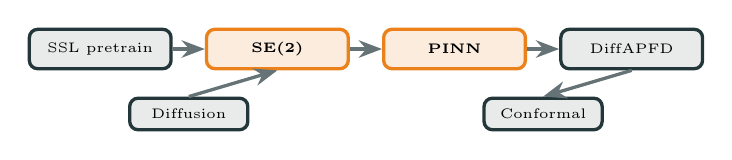
\begin{tikzpicture}[scale=0.75]
\begin{scope}[xscale=1.2, yscale=1.1]
  \node[draw=mDarkTeal, very thick, rounded corners=3pt, fill=mDarkTeal!10, minimum height=0.5cm, minimum width=1.8cm, align=center, font=\tiny] (a) at (0, 1) {SSL pretrain};
  \node[draw=accent, very thick, rounded corners=3pt, fill=accent!15, minimum height=0.5cm, minimum width=1.8cm, align=center, font=\tiny\bfseries] (b) at (2.5, 1) {SE(2)};
  \node[draw=accent, very thick, rounded corners=3pt, fill=accent!15, minimum height=0.5cm, minimum width=1.8cm, align=center, font=\tiny\bfseries] (c) at (5, 1) {PINN};
  \node[draw=mDarkTeal, very thick, rounded corners=3pt, fill=mDarkTeal!10, minimum height=0.5cm, minimum width=1.8cm, align=center, font=\tiny] (d) at (7.5, 1) {DiffAPFD};
  \node[draw=mDarkTeal, very thick, rounded corners=3pt, fill=mDarkTeal!10, minimum height=0.4cm, minimum width=1.5cm, align=center, font=\tiny] (e) at (1.25, 0) {Diffusion};
  \node[draw=mDarkTeal, very thick, rounded corners=3pt, fill=mDarkTeal!10, minimum height=0.4cm, minimum width=1.5cm, align=center, font=\tiny] (f) at (6.25, 0) {Conformal};
  \draw[-{Stealth}, very thick, mDarkTeal!70] (a) -- (b);
  \draw[-{Stealth}, very thick, mDarkTeal!70] (b) -- (c);
  \draw[-{Stealth}, very thick, mDarkTeal!70] (c) -- (d);
  \draw[-{Stealth}, very thick, mDarkTeal!70] (e.north) -- (b.south);
  \draw[-{Stealth}, very thick, mDarkTeal!70] (d.south) -- (f.north);
\end{scope}
\end{tikzpicture}
\par}

\vspace{0.3em}
\scriptsize
\begin{tabular}{p{2.2cm} p{2.2cm} p{2.2cm} p{2.2cm}}
\centering\textbf{SE(2)} & \centering\textbf{PINN} & \centering\textbf{DiffAPFD} & \centering\textbf{Conformal} \\
$\Delta$=0 invariant & 5.6$\times$ violation drop & Low variance $\sigma$ & APFD coverage bound
\end{tabular}

\vspace{0.5em}
\begin{block}{Target}
\scriptsize
\[
\boxed{\text{APFD} \ge 0.820 \pm 0.010 \text{ with all guarantees stacked}}
\]
\end{block}
\end{frame}

\begin{frame}{Key Takeaways}
\begin{center}
\vspace{-0.5em}
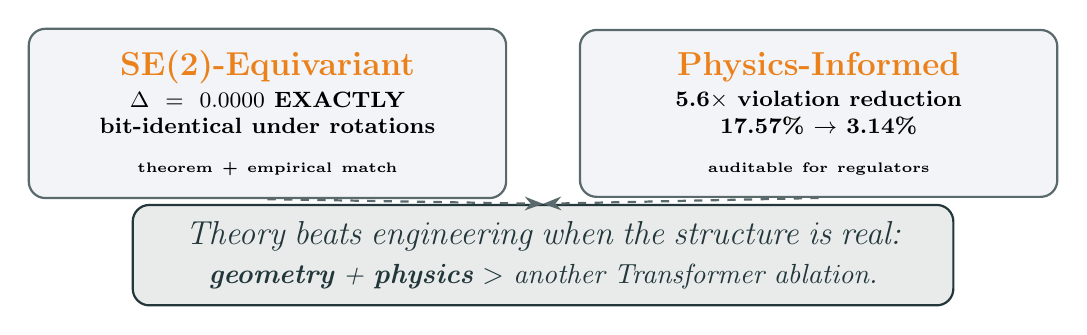
\begin{tikzpicture}[
  card/.style={fill=softgray, draw=navymid, thick, rounded corners=6pt, inner sep=8pt, align=center}
]
  \node[card, text width=5.5cm, minimum height=1.8cm] (acc) at (-3.5, 0) {
    \large\bfseries\textcolor{accent}{SE(2)-Equivariant}\\[2pt]
    \footnotesize
    $\Delta = 0.0000$ EXACTLY\\
    bit-identical under rotations\\[2pt]
    \tiny theorem + empirical match
  };

  \node[card, text width=5.5cm, minimum height=1.8cm] (spd) at (3.5, 0) {
    \large\bfseries\textcolor{accent}{Physics-Informed}\\[2pt]
    \footnotesize
    5.6$\times$ violation reduction\\
    17.57\% $\to$ 3.14\%\\[2pt]
    \tiny auditable for regulators
  };

  \node[fill=mDarkTeal!10, draw=mDarkTeal, thick, rounded corners=6pt, inner sep=6pt, text width=10cm, align=center]
    (q) at (0, -1.8) {
    \large\itshape\textcolor{mDarkTeal}{Theory beats engineering when the structure is real:}\\[2pt]
    \normalsize\textcolor{mDarkTeal}{\textbf{geometry} + \textbf{physics} $>$ another Transformer ablation.}
  };

  \draw[-{Stealth}, thick, navymid, dashed] (acc.south) -- (q.north);
  \draw[-{Stealth}, thick, navymid, dashed] (spd.south) -- (q.north);
\end{tikzpicture}
\end{center}
\end{frame}

\begin{frame}[standout]
\centering
\vspace{0.8em}
\Huge Thank You!\\[0.5em]
\Large \textcolor{accent}{Questions?}

\vspace{1.5em}
\normalsize
\textbf{Theory-Driven Test Prioritization for Self-Driving Car Simulators}\\[0.3em]
\scriptsize
Đào Sỹ Duy Minh \quad $\cdot$ \quad Trần Chí Nguyên \quad $\cdot$ \quad Huỳnh Trung Kiệt\\
University of Science, VNU-HCM \quad $\cdot$ \quad NeurIPS 2026
\end{frame}

\end{document}
